\newpage
\section{Results \& Discussion}\label{sec:results}
\subsection{Matching}
\subsection{Coordinate Matching}
\label{sec:coordinate_calibration}

\begin{wrapfigure}[39]{r}{0.5\textwidth}
    \vspace{-3cm}
    \centering
    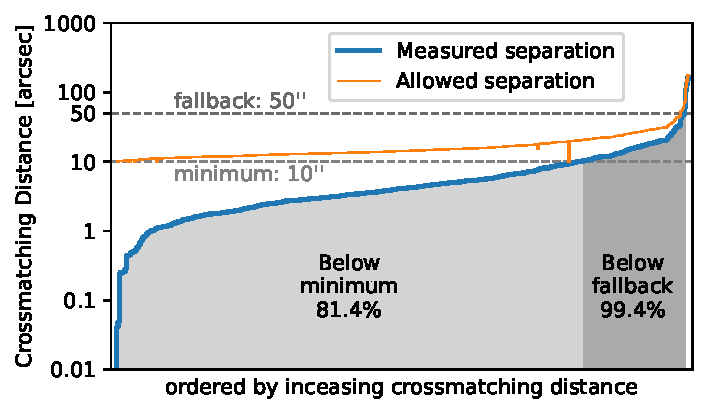
\includegraphics[width=\linewidth]{figures/nea_coordinate_calibration.pdf}
    \caption{Calibration of coordinate crossmatching for NEA using SIMBAD IDs to crossmatch with HPICxLIFEcat. The separations between matched HPICxLIFEcat input stars and NEA catalog positions are plotted in increasing order and the algorithm’s 10'' minimum matching tolerance and 50'' fallback threshold overlaid to illustrate how the observed IDs fall within the adopted angular acceptance. The remaining 0.6\% above the fallback threshold are also coordinate matched due to the proper-motion-sensitive search radius.}
    \label{fig:nea_coord_cal}
    \vspace{0.5cm}
    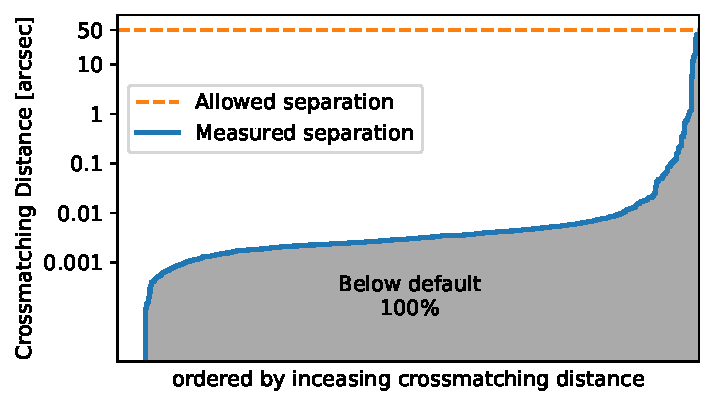
\includegraphics[width=1\linewidth]{figures/emc_coordinate_calibration.pdf}
    \caption{Calibration of coordinate crossmatching for EMC using ID crossmatches showing the measured angular separations for matched HPICxLIFEcat stars with the 50'' matching tolerance annotated to demonstrate that all ID-based matches remain within the adopted acceptance radius}
    \label{fig:emc_coord_cal}
    \vspace{0.5cm}
    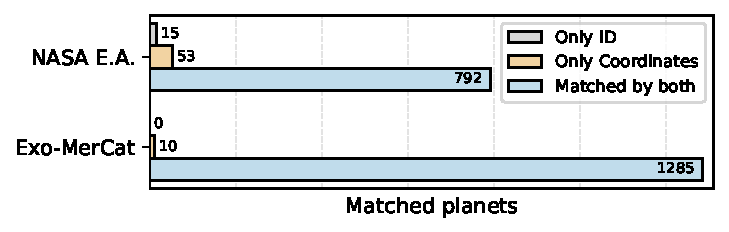
\includegraphics[width=\linewidth]{figures/crossmatch_yield.pdf}
    \caption{Yield of matched planets for the NASA Exoplanet Archive and Exo-MerCat catalogs, categorized by which methods the match was established.}
    \label{fig:yield}
\end{wrapfigure}



The NASA exoplanet archive (shortened here to NEA) is by far the most cited exoplanet catalog and thus deserves special attention among the input sources. NEA's coordinates are assembled from many different sources and the coordinate epoch can be read or estimated from the source they list for the entry. As can be seen in \cref{fig:nea_coord_cal}, using the proper-motion-aware formula on a set of ID-matched stars, we achieve a matching accuracy of 100\%. Neglecting the proper motion correction, we see that 50'' is a reasonable threshold for matching when that option is not available. By comparing the distances to the next-nearest neighbors in the HPICxLIFEcat catalog, we also find that 50'' leads to no predicted false positives.




Exo-MerCat does not carry columns for proper motion, thus only a "default" search radius can be applied. Despite this, as is observed in \cref{fig:emc_coord_cal}, the average crossmatching distance between HPICxLIFEcat and Exo-MerCat is generally around two orders of magnitude smaller than the average crossmatching distance between HPICxLIFEcat and NEA (c.f. \cref{fig:nea_coord_cal}). This relates to the fact that Exo-MerCat takes its coordinates from SIMBAD, which for HPICxLIFEcat is also the primary data source. In opposition, NEA carries its own heterogeneously sourced coordinate entries, many of which do not even carry the same epochs and sometimes reach back to the mid 20th century. As before, the likelihood of false positives stays low due to the low density across the sky. 




\subsection{Combined Matching}
As shown in \cref{fig:yield}, coordinate-only matching proves to be the edge case, as matching with NEA and Exo-MerCat primarily results in matches based on linked identifiers. As expected, Exo-MerCat matches are almost a superset of the NEA matches. The only exceptions are high-mass directly imaged planets that were removed by Exo-MerCat's BD-removal step. The lower count of only-coordinate matches can primarily be explained by Exo-MerCat's internal alternate ID handling, which covers more cases than the one implemented for SIMBAD in this project.

\subsection{Population Analysis}
Exo-MerCat assembles the largest published list of exoplanets, and is thus very useful in gaining a sense of the broader known planet population. In \cref{fig:pop_distr} we can see certain features of the diagram correspond to specific parts of the exoplanet population (Note that part of the data was taken from post-Exo-MerCat enrichment computations, a version without can be found in \cref{fig:pop_distr_nocomp} in appendix \cref{appddx:nocomp}): For example the "bulge" on the top right (high insolation, high radius) represents the hot jupiter type planets. The long thin strand pointing downwards on the right half of the plot are wide-separation planets observed via direct imaging. The bunching around $\qty{E1}{\Rearth}$ is likely a consequence of the \textcite{ChenKipping2017} power law's local maximum around that value, which NEA uses internally to compute radii from masses when their missing \cite{NasaExoplanetArchive}. 

\begin{figure}[ht]
    \centering
    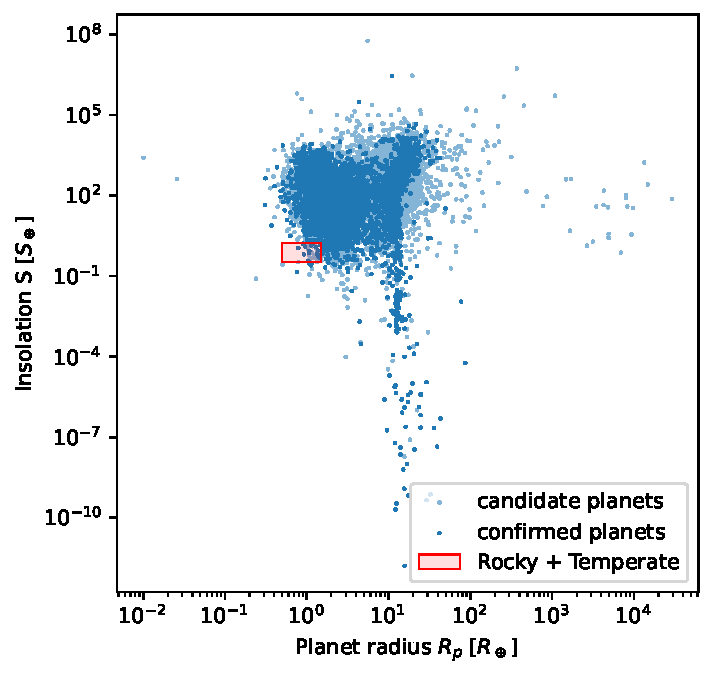
\includegraphics[width=0.72\textwidth]{figures/radius_insolation_distribution.pdf}
    \caption{Distribution of the enriched Exo-MerCat exoplanet population in terms of planet-radius insolation (contains parameter computations). Confirmed planets are drawn in the darker shade and unconfirmed candidates in the lighter shade. The red rectangle marks the rocky-and-temperate selection region adopted in this work, spanning a radius of $0.5$--$1.5\,R_\oplus$ and an incident stellar flux of $0.35$--$1.7\,S_\oplus$.}
    \label{fig:pop_distr}
\end{figure}

We can compare the overall distribution with just the distribution of planets matched by HPICxLIFEcat, here done in heatmap form to better assess how many planets share similar parameters, presented in \cref{fig:pop_heatmap} (and a decomposition into the spectral categories of the same heatmap in appendix \cref{appdx:spectral_category} \cref{fig:pop_heatmap_spectral}). Note that the feature of hot jupiters is absent in the left side since low-mass stars are known to rarely host hot jupiters \cite{Ganetal2023}. Because very-low-luminosity stats are highly abundant in our solar neighborhood, they dominate the HPICxLIFEcat stellar population and host nearly all of these planets. We are not excluding any planets from being classified as temperate and rocky by undershooting the $0.5\Rearth$ boundary, which is likely due to observational biases against low-mass/radius and comparatively long-period planets \cite{Guyon2017}.


\begin{figure}[ht]
    \centering
    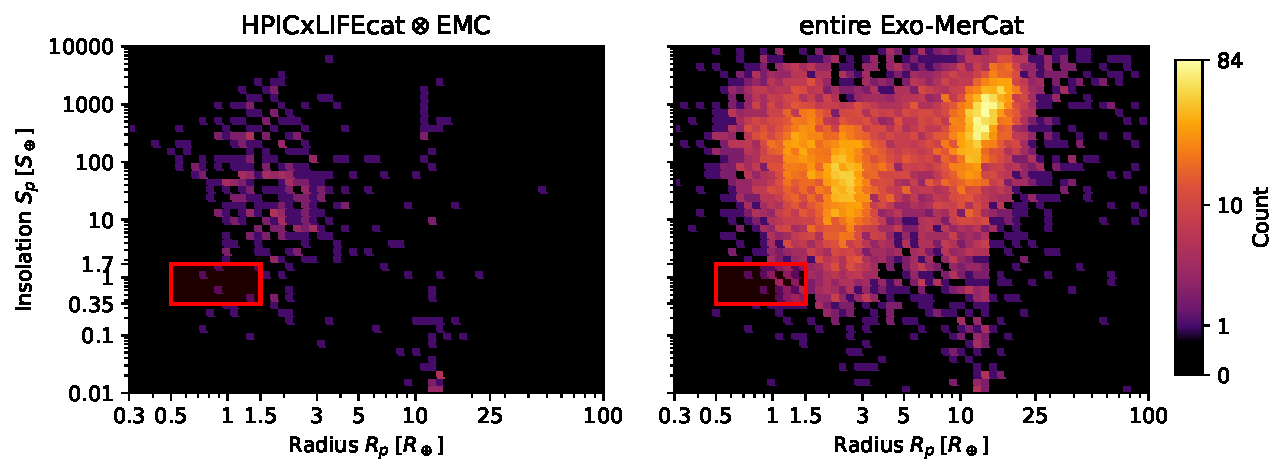
\includegraphics[width=\textwidth]{figures/radius_insolation_heatmap.pdf}
    \caption{Two-dimensional number density heatmap of the known exoplanet population w.r.t planet-radius and insolation comparing the distributions in Exo-MerCat and Exo-MerCat matched to HPICxLIFEcat. The red rectangle marks the same rocky-and-temperate selection region as in \cref{fig:pop_distr}, spanning $0.5$--$1.5\,R_\oplus$ and $0.35$--$1.7\,S_\oplus$. A breakdown of the same distribution by host spectral category is given in \cref{fig:pop_heatmap_spectral}.}
    \label{fig:pop_heatmap}
\end{figure}

Particularly interesting to the LIFE mission is the population of rocky habitable zone planets. We categorize stars into three categories based on their spectral type: Sun-like (F0V-K5V), Low-luminosity (K6V-M2V), and Very-low-luminosity (M3V-M9V). All left over spectral types and non-main-sequence stars are grouped as "Other".  Furthermore, working with the definition \cref{lab:hz_def} we differentiate between two kinds planets can be classified as rocky and temperate. The first one is "Confirmed", when its published values lie within our definition. "Uncertain" means the planet might be rocky and temperate in the sense that it is either a candidate planet meeting the requirements or a planet whose measurement error in the relevant quantities makes the allowed parameter range overlap with our definition of habitable. The full list of rocky, temperate planet candidates underlying \cref{fig:rocky_temp_yield} is given in \cref{appdx:rocky_temp_tables}: \cref{tab:rocky_temp_table} for the distance-limited HPIC$\times$LIFEcat crossmatched sample and \cref{tab:rocky_temp_table_full} for the entire Exo-MerCat catalog.

\begin{figure}[H]
    \centering
    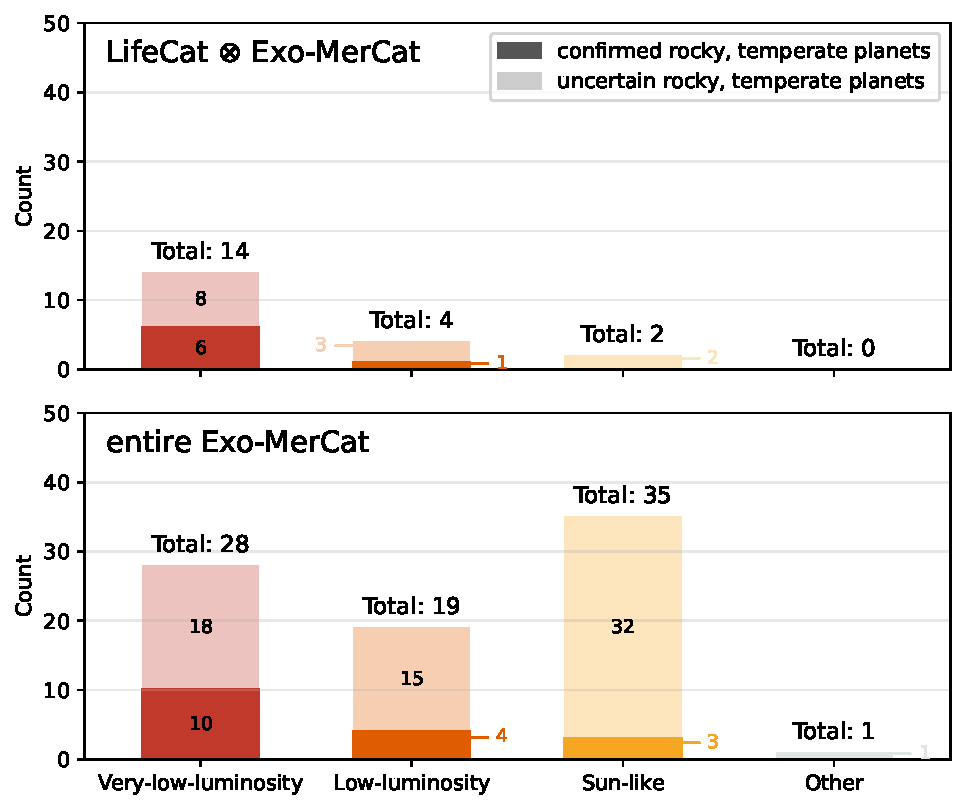
\includegraphics[width=0.9\textwidth]{figures/rocky_temperate_yield.pdf}
    \caption{Yield of rocky, temperate planet candidates by host-star spectral category, using the same selection region as \cref{fig:pop_distr} and \cref{fig:pop_heatmap} (radius $0.5$--$1.5\,R_\oplus$, insolation $0.35$--$1.7\,S_\oplus$). A planet is counted as confirmed (dark shading) if its central-value radius and insolation both fall inside the box and it is a confirmed planet, and as uncertain if the box is met only within the uncertainty of the radius/insolation uncertainty interval, or if the central values fall inside the box but the planet is not confirmed. The top panel shows the distance-limited HPIC$\times$LIFEcat sample crossmatched with Exo-MerCat (20 candidates in total), the bottom panel the entire Exo-MerCat catalog (83 candidates in total). The full list of candidates is given in Appendix \cref{appdx:rocky_temp_tables}.}
    \label{fig:rocky_temp_yield}
\end{figure}


\subsection{Outlook}
This project stands as a tool to quickly and reliably match known exoplanets to any stellar catalog, which can be used in the future for yield estimates similar to how a simulated exoplanetary catalog was employed by \textcite{life4}. Furthermore, this work may be used for studies similar to \citetitle{Life10} by \textcite{Life10} by providing a quick and repeatable way of selecting potentially habitable planets to then study on a case by case basis.

On the enrichment side, by comparing and potentially adopting some of \citetitle{Bohl_2026} by \textcite{Bohl_2026} methods, better enrichment pathways can be exploited to further increase the number of paper-sourced parameters and use more accurate methods for inferring missing parameters to get a better sense of the broader exoplanet population.

